\documentclass[conference]{IEEEtran}
\IEEEoverridecommandlockouts

\usepackage{cite}
\usepackage{amsmath,amssymb,amsfonts}
\usepackage{amsthm}
\usepackage{algorithmic}
\usepackage{textcomp}
\usepackage{xcolor}
\usepackage{graphics}
\usepackage{textcomp}
\usepackage{comment}
\usepackage{tabularx}
\usepackage{breqn}
\usepackage{url}
\usepackage{listings}
\usepackage{threeparttable}
\usepackage[linesnumbered,ruled]{algorithm2e}
\usepackage{color}
\usepackage{soul}
\usepackage{multirow}

\setcounter{topnumber}{100}
\setcounter{bottomnumber}{100}
\setcounter{totalnumber}{100}
\renewcommand{\textfraction}{0.0}
\renewcommand{\topfraction}{1.0}

% code style setting
\lstset{
    %プログラム言語(複数の言語に対応,C,C++も可)
    language = c,
    %枠外に行った時の自動改行
    breaklines = true,
    %自動開業後のインデント量(デフォルトでは20[pt])	
    breakindent = 5pt,
    %標準の書体
    basicstyle = \ttfamily\scriptsize,
    %basicstyle = {\small}
    %コメントの書体
    commentstyle = {\itshape \color[cmyk]{1,0.4,1,0}},
    %関数名等の色の設定
    % classoffset = 0,
    %キーワード(int, ifなど)の書体
    keywordstyle = {\bfseries \color[cmyk]{0,1,0,0}},
    %""で囲まれたなどの"文字"の書体
    % stringstyle = {\ttfamily \color[rgb]{0,0,1}},
    %枠 "t"は上に線を記載, "T"は上に二重線を記載
    %他オプション:leftline,topline,bottomline,lines,single,shadowbox
    frame = TB,
    %frameまでの間隔(行番号とプログラムの間)
    framesep = 1pt,
    %行番号の位置
    numbers = left,
    %行番号の間隔
    stepnumber = 1,
    %右マージン
    xrightmargin=0pt,
    %左マージン
    xleftmargin=0pt,
    %行番号の書体
    numberstyle = \scriptsize,
    %タブの大きさ
    tabsize = 4,
    %キャプションの場所("tb"ならば上下両方に記載)
    captionpos = t,
    columns=[l]fullflexible,
    escapeinside={(*}{*)}
}

\bibliographystyle{unsrt}

\def\BibTeX{{\rm B\kern-.05em{\sc i\kern-.025em b}\kern-.08em
    T\kern-.1667em\lower.7ex\hbox{E}\kern-.125emX}}


%%% Original command %%%
\sethlcolor{yellow}
% \newcommand{\todo}[1]{\hl{\textbf{TODO:} #1}}
\newcommand{\hack}[1]{\hl{\textbf{HACK:} #1}}
\newcommand{\todo}[1]{}
% \newcommand{\hack}[1]{}

\newcommand{\la}[0]{$\leftarrow$ }
\newcommand{\ch}[0]{\checkmark}

\newcommand{\tabml}[1]{\hspace{-2.2mm}\begin{tabular}{l} #1 \end{tabular}}


%%% Original function %%%
\def\MR#1#2{\multirow{#1}{*}{#2}}
\def\MC#1#2#3{\multicolumn{#1}{#2}{#3}}


%%% Start paper %%%
\begin{document}

\title{MRDAG-Gen: Multi-rate DAG Generator}
\maketitle

\author{
    \IEEEauthorblockN{Atsushi Yano and Takuya Azumi}
    \IEEEauthorblockA{\textit{Graduate School of Science and Engineering,} \\ \textit{Saitama University}}
}

\begin{abstract}
    \todo{}
\end{abstract}


\begin{IEEEkeywords}
    DAG, Random generation tool, Multi-rate systems
\end{IEEEkeywords}

\section{Introduction}
\label{sec: introduction}

\cite{10.1145/3381847}
\todo{}


\section{System model}
\label{sec: system_model}


\begin{figure}[tb]
    \centering
    \scalebox{1.0}{
        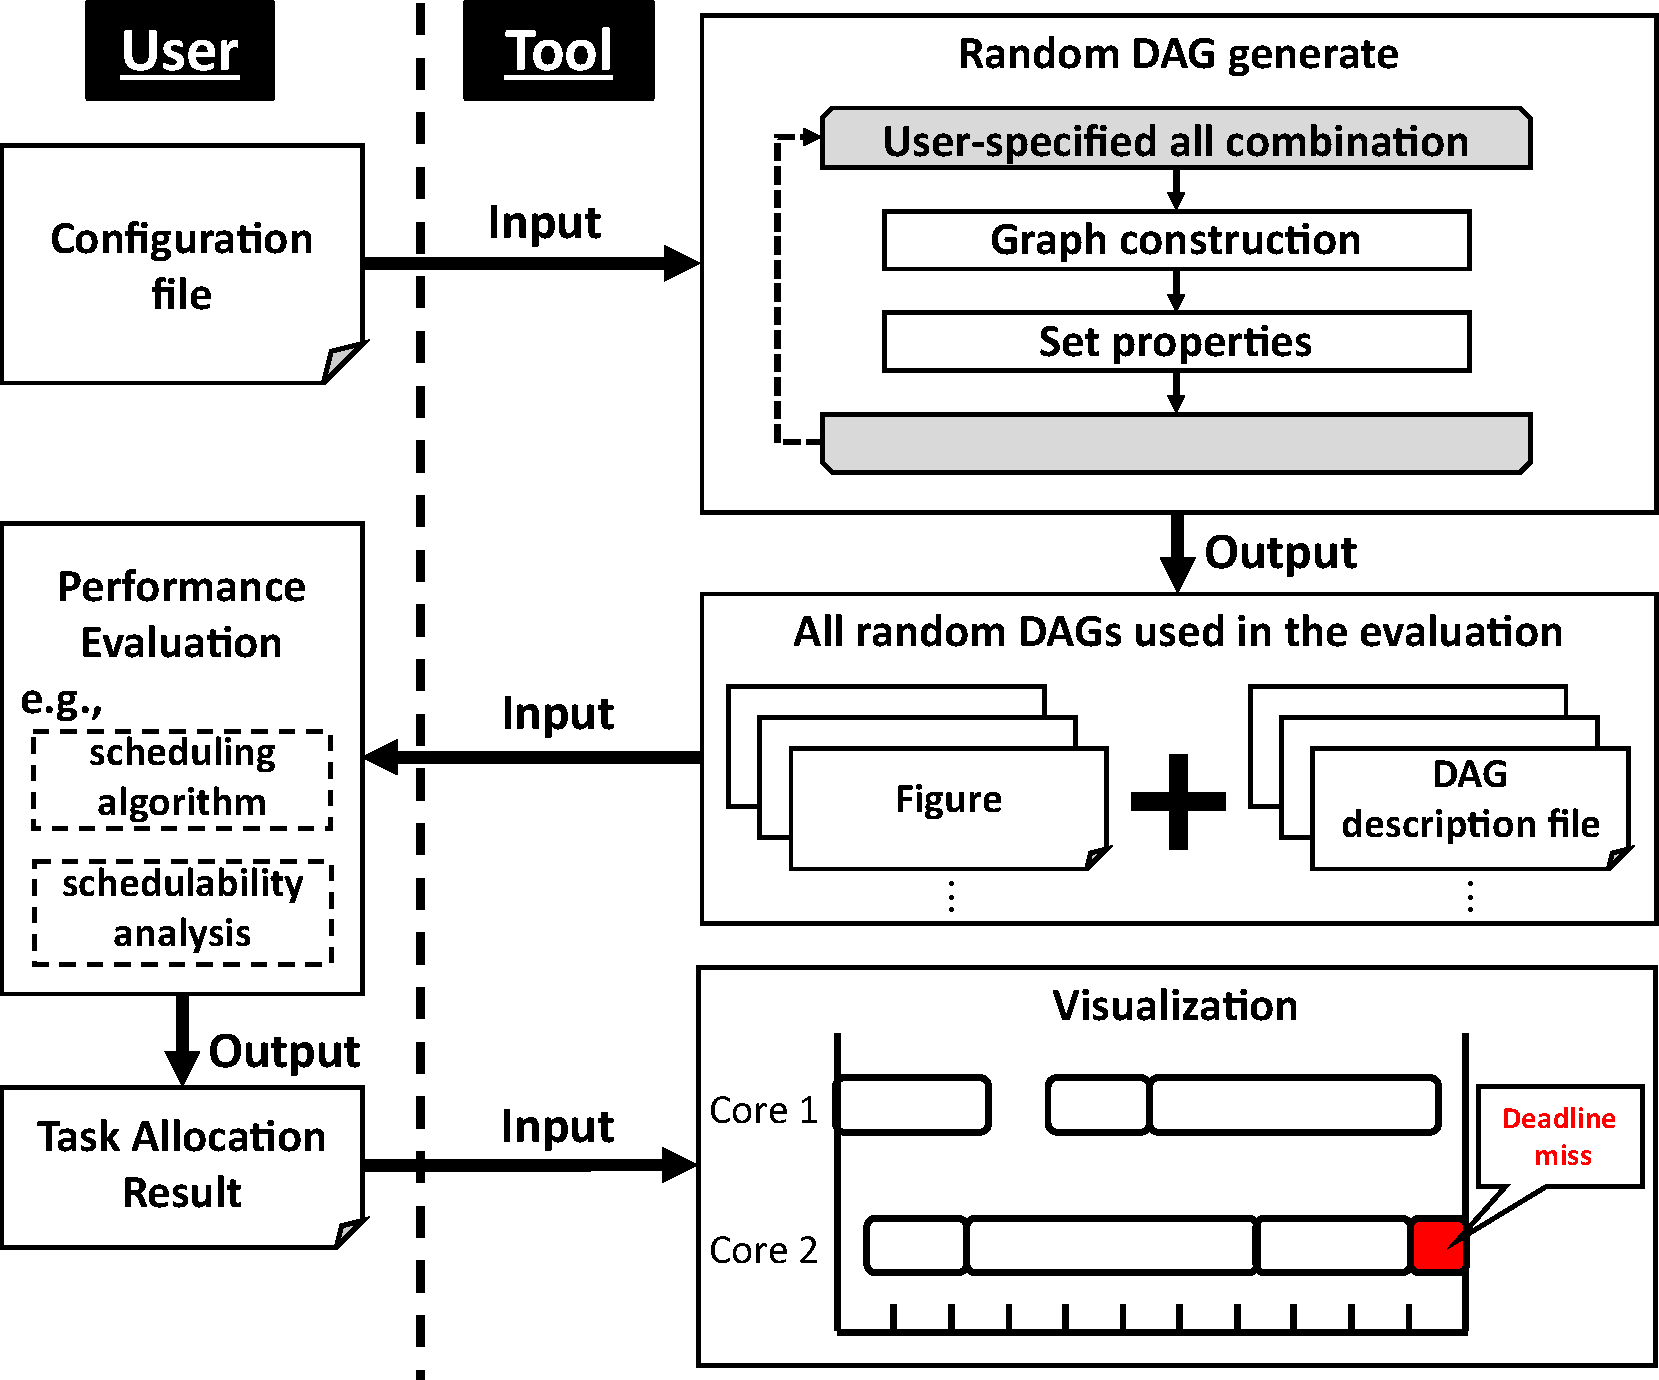
\includegraphics[width=\linewidth]{./src/figure/system_model.pdf}
    }
    \caption{System model.}
    \label{fig: system_model}
\end{figure}


\begin{table}[tb]
    \centering
    \caption{DAG Notations}
    \label{tab: dag_notations}
    \renewcommand{\arraystretch}{1.2}
    \scalebox{1.0}{
        \begin{tabular}{c|l}\hline\hline
            $G$            & DAG                                            \\ \hline
            $V$            & Set of all nodes of $G$                        \\ \hline
            $|V|$          & Total number of nodes of $G$                   \\ \hline
            $E$            & Set of all edges of $G$                        \\ \hline
            $\tau_i$       & $i$-th Node                                    \\ \hline
            $C_i$          & WCET of $\tau_i$                               \\ \hline
            $e_{i,j}$      & Edge between $\tau_i$ and $\tau_j$             \\ \hline
            $comm_{i,j}$   & Communication time of $e_{i,j}$                \\\hline
            $CCR$          & CCR of $G$                                     \\\hline
            $D$            & End-to-end deadline                            \\ \hline
            $\tau^{tm}_i$  & $i$-th timer-driven node                       \\ \hline
            $\phi_i$       & Offset of $\tau^{tm}_i$                        \\ \hline
            $T_i$          & Execution period of $\tau^{tm}_i$              \\ \hline
            $d_i$          & Relative deadline of $\tau^{tm}_i$             \\ \hline
            $u_i$          & Utilization of $\tau^{tm}_i$                   \\\hline
            $U$            & Total Utilization of $G$                       \\\hline
            $\Gamma_i$     & $i$-th chain                                   \\\hline
            $|\Gamma|$     & Total number of chains of $G$                  \\\hline
            $C_{\Gamma_i}$ & WCET of $\Gamma_i$                             \\ \hline
            $u_{\Gamma_i}$ & Utilization of $\Gamma_i$                      \\ \hline
            $T_{\Gamma_i}$ & Period of head timer-driven node of $\Gamma_i$ \\ \hline
        \end{tabular}
    }
\end{table}


This section represents the system model, as shown in Fig.~\ref{fig: system_model}.
Section~\ref{ssec: single_rate_dag} describes the basic single-rate DAG.
Section~\ref{ssec: multi_rate_dag} explains a multi-rate DAG.
The DAG notations used in this paper are listed in Table~\ref{tab: dag_notations}.


\subsection{Single-rate DAG}
\label{ssec: single_rate_dag}

Single-rate DAGs are DAGs with either a single entry node or all entering at the same time, used in real-time application \cite{zhao2020dag}, cyber-physical systems \cite{senapati2021hmds} and cloud computing \cite{kaur2020deep}, and so forth.
Here, the entry node represents the input to the system (e.g., a sensor event or a command from the user), and the exit node represents the final output from the system.

A DAG consists of a node set and an edge set, denoted $G = (V, E)$.
Nodes represent tasks in the system, and edges represent communication and dependencies between nodes or priority constraints.
$V$ is the set of all nodes, expressed as $V = \{\tau_1, ..., \tau_{|V|}\}$, where $|V|$ is the total number of nodes.
Each node has a worst-case execution time (WCET), and the WCET of $\tau_i$ is denoted as $C_i$.
$E$ is the set of all edges, where each edge $e_{i,j} \in E$ represents communication between $\tau_i$ and $\tau_j$ and a priority constraint.
When $e_{i,j}$ exists in the DAG, $\tau_j$ cannot be executed until $\tau_i$ has completed its execution and the output of $\tau_i$ has arrived.
If the communication time is given as an assumption, the communication time at $e_{i,j}$ is denoted as $comm_{i, j}$.
The ratio of the sum of the communication times of all edges to the sum of the execution times of all nodes is called the communication-to-computation ratio (CCR) and is defined by Eq~\ref{eq: ccr}.

\begin{equation}
    \label{eq: ccr}
    CCR = \frac{\sum\limits_{e_{i,j} \in E}comm_{i, j}}{\sum\limits_{\tau_i \in V}C_i}
\end{equation}

An end-to-end deadline $D$ is set at the exit node when it is necessary to guarantee the safety of hard real-time systems \cite{yano2021work} or the quality of service of cloud computing \cite{zhang2020efficient}.


\subsection{Multi-rate DAG}
\label{ssec: multi_rate_dag}

A multi-rate DAG is a DAG that contains multiple nodes that are triggered at different periods.
Here, the definitions of nodes and edges in a multi-rate DAG are the same as those shown in Section~\ref{ssec: single_rate_dag}.
Multi-rate DAGs can be broadly classified into two categories: (i) DAGs in which all nodes are timer-driven nodes, as in automotive systems \cite{kordon2020evaluation, verucchi2020latency}, and (ii) DAGs that combine a chain consisting of timer-driven nodes and a chain of linked event-driven nodes, as in self-driving systems \cite{choi2021picas, tang2020response}.


\subsubsection{Multi-rate DAG consisting of only timer-driven nodes}
\label{sssec: dag_only_timer}

Each timer-driven node in these multi-rate DAGs is denoted by $\tau^{tm}_i$, and $\tau^{tm}_i$ is characterized by the tuple $(\phi_i, Ci, Ti, di)$.
$\phi_i$, $T_i$, and $d_i$ represent the offset, execution period, and relative deadline, respectively.
For DAGs that consider timer-driven nodes, every timer-driven node has a relative deadline of $T_i$ time units indicating that every job of $\tau^{tm}_i$ has an absolute deadline at $T_i$ time units after its release \cite{yang2020mixed, cho2021conditionally}.
Such a time constraint is called an implicit deadline, and MRDAG-Gen generates DAGs that consider implicit deadlines.

The utilization of $\tau^{tm}_i$ is denoted as $u_i$ calculated by $u_i = C_i / T_i$.
The total utilization $U$ of a DAG consisting only of timer-driven nodes is defined by Eq.~\ref{eq: total_utilization_only_timer}.

\begin{equation}
    \label{eq: total_utilization_only_timer}
    U = \sum_{\tau^{tm}_i \in V}u_i
\end{equation}


\begin{figure}[tb]
    \centering
    \scalebox{1.0}{
        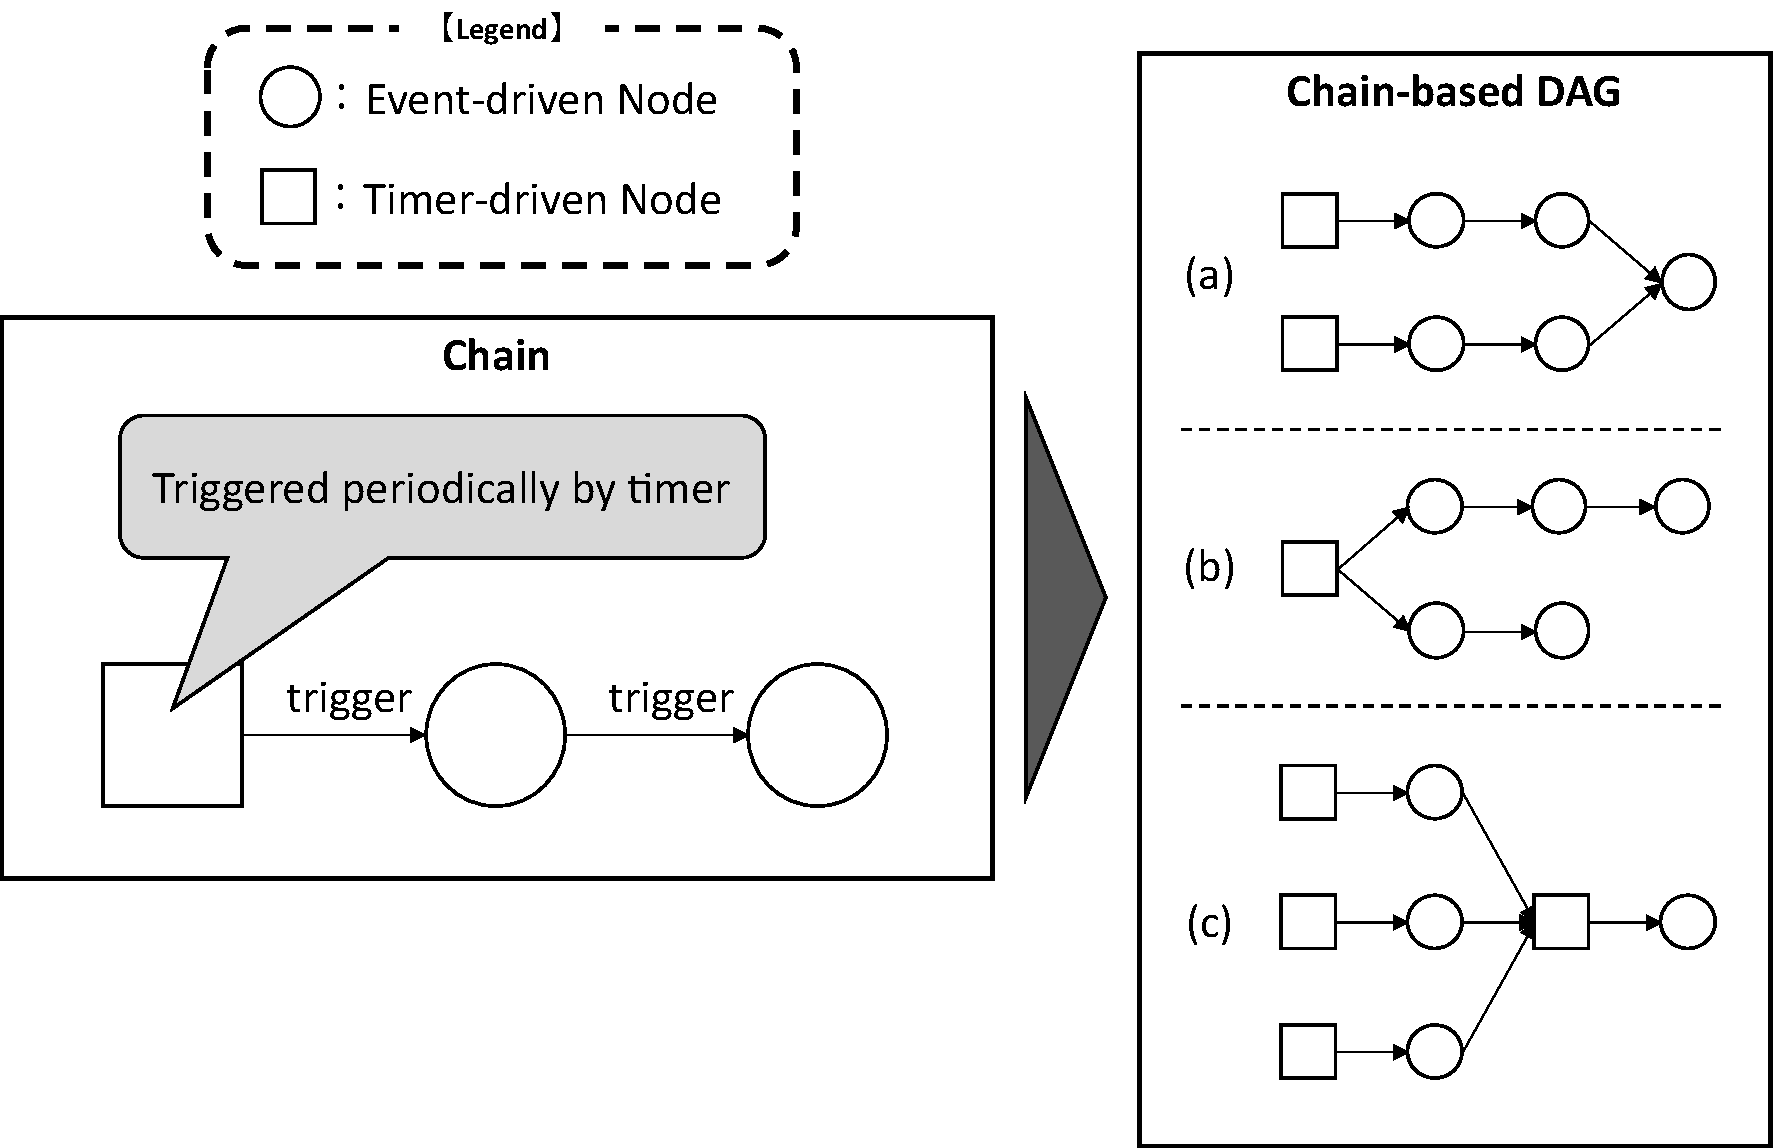
\includegraphics[width=\linewidth]{./src/figure/chain_based_dag.pdf}
    }
    \caption{Multi-rate DAGs consisting of chains}
    \label{fig: chain_dag}
\end{figure}


\subsubsection{Chain-based multi-rate DAG}
\label{sssec: dag_chain}

In the latest multi-rate systems, DAGs consisting of the chain shown in Fig.~\ref{fig: chain_dag} are considered.
Each chain $\Gamma_i$ is denoted as $\Gamma_i = \{\tau^{tm}_i, \tau_k, ..., \tau_{|\Gamma_i|}\}$, where $|\Gamma_i|$ is the number of nodes that compose $\Gamma_i$.
The head $\tau^{tm}_i$ in the chain is triggered periodically, and subsequent event-driven nodes are triggered by their direct predecessors.
This definition is also used in existing studies \cite{choi2020chain, tang2020response}.
The WCET of $\Gamma_i$ is denoted by $C_{\Gamma_i}$ and defined in Eq.~\ref{eq: wcet_chain}.

\begin{equation}
    \label{eq: wcet_chain}
    C_{\Gamma_i} = \sum_{\tau_i \in \Gamma}C_i
\end{equation}

Since the chain is executed dependent on the period of the head timer-driven node, the utilization of the chain $u_{\Gamma_i}$ is calculated by Eq~\ref{eq: chain_utilization}.

\begin{equation}
    \label{eq: chain_utilization}
    u_{\Gamma_i} = \frac{C_{\Gamma_i}}{T_{\Gamma_i}}
\end{equation}

\noindent Here, $T_{\Gamma_i}$ is the period of the head timer-driven node $\tau^{tm}_i$ of the chain.
The total utilization of the chain-based multi-rate DAG is defined by Eq~\ref{eq: chain_total_utilization}.

\begin{equation}
    \label{eq: chain_total_utilization}
    U = \sum_{\Gamma_i \in V}u_{\Gamma_i}
\end{equation}

The chain-based multi-rate DAGs exist mainly in robot operating system (ROS)-based systems \cite{casini2019response, choi2021picas}.
In a typical ROS-based system, a self-driving system (e.g., Autoware \cite{future}), different sensor data are processed and merged by multiple chains to output the final command.
When modeling ROS-based systems as DAGs, it is necessary to consider DAGs where multiple chains merge at exit nodes ((a) in Fig.~\ref{fig: chain_dag}), where the chain branches ((b) in Fig.~\ref{fig: chain_dag}), and where multiple chains are vertically linked ((c) in Fig.~\ref{fig: chain_dag}).
MRDAG-Gen can generate all these DAGs by using various parameters.


\section{Design and Implementation}
\label{sec: design_implementation}

\todo{}


\section{Evaluation using case study}
\label{sec: evaluation_case_study}

\todo{}


\section{Related work}
\label{sec: related_work}

This section describes existing random DAG generation tools and existing studies using random DAGs and compares them with MRDAG-Gen.
Table~\ref{tab: comparison} shows a comparison of MRDAG-Gen with existing methods.

\begin{table}[tb]
    \centering
    {

        \caption{MRDAG-Gen vs existing methods}
        \label{tab: comparison}
        \renewcommand{\arraystretch}{1.2}
        \scalebox{0.8}{
            \begin{tabular}{c|cccccc} \hline\hline
                                                           & RMD & RPU & RDT & RTE & OCG \\\hline\hline
                DAGEN \cite{amalarethinam2011dagen}        &     &     & \ch &     &     \\\hline
                MRTG \cite{ashish2016modular}              &     &     & \ch &     &     \\\hline
                TGFF \cite{tgff}                           &     &     & \ch &     &     \\\hline
                GGen \cite{cordeiro2010random}             & \ch &     & \ch &     &     \\\hline
                Kordon et al. \cite{kordon2020evaluation}  & \ch &     &     &     &     \\\hline
                Yang et al.   \cite{yang2020mixed}         & \ch & \ch &     &     &     \\\hline
                Gunzel et al. \cite{gunzel2021suspension}  & \ch & \ch &     &     &     \\\hline
                Ueter et al. \cite{ueter2021hard}          & \ch & \ch &     &     &     \\\hline
                Dong et al. \cite{dong2019efficient}       & \ch & \ch &     &     &     \\\hline
                He et al. \cite{he2021response}            & \ch & \ch &     &     &     \\\hline
                Voronov et al. \cite{voronov2021ai}        & \ch & \ch &     &     &     \\\hline
                Verucchi et al. \cite{verucchi2020latency} & \ch & \ch &     &     &     \\\hline
                Klaus et al. \cite{klaus2021constrained}   & \ch & \ch &     &     &     \\\hline
                Tang et al. \cite{tang2020response}        & \ch & \ch &     & \ch &     \\\hline
                Choi et al. \cite{choi2021picas}           & \ch & \ch &     & \ch &     \\\hline
                MRDAG-Gen                                  & \ch & \ch & \ch & \ch & \ch \\\hline
            \end{tabular}
        }
        \begin{tablenotes}[normal]{
                \item {RMD}: Random generation of multi-rate DAGs
                \item {RPU}: Random property settings based on total utilization
                \item {RDT}: Random DAG generation tool
                \item {RTE}: Random generation of chain-based multi-rate DAGs
                \item {OCG}: One-command batch generation of random DAGs
            }
        \end{tablenotes}
    }
\end{table}


\subsection{Random DAG generation with unique implementation}
\label{sec: random_tool}

Random DAG generation tools provide reliability and reproducibility for evaluations of scheduling and latency analysis studies.
TGFF \cite{tgff} is the first tool proposed for this purpose and has been used to evaluate most recent studies \cite{roeder2021energy, fard2021analytical, wu2021evolutionary, costa2021extracting}.
TGFF determines the shape of a DAG primarily by specifying either or both the maximum and minimum input degree and maximum (first) output degree for a single node (the {\it Fan-in/Fan-out} method).
TGFF can quickly generate many DAGs, and the task set can be easily reproduced by other researchers by inputting the same parameters.
However, TGFF was released in 1998 and has many problems, such as its output format (.tgff), which is difficult to handle, and it cannot generate the multi-rate DAGs.

GGen \cite{cordeiro2010random} is a unified implementation of classical task graph generation methods used in the scheduling domain.
GGen allows the user to add properties such as the execution period and the communication time to nodes and edges after generating DAGs using a user-specified generation method.
However, GGen does not allow constraints to be specified between different properties, such as implicit deadlines (i.e., the execution time of a node must not exceed its period).
Therefore, users with such requirements must adjust these values themselves.

Other random DAG generation tools such as DAGGEN \cite{amalarethinam2011dagen} and MRTG \cite{ashish2016modular} have also been proposed.
DAGGEN generates random workflow applications by specifying the node load balancing, edge connection probability, and workflow shape.
MRTG is a random DAG generation tool with a module-based implementation for user extensibility.
However, these tools are not capable of generating multi-rate DAGs.
Conversely, MRDAG-Gen can flexibly generate multi-rate DAGs of various types.
In addition, MRDAG-Gen can automatically set properties calculated by multiple values such as CCR and the total utilization.


\subsection{Unique implementation of random DAG generation}

This section presents existing studies in which the authors generated random DAG sets to evaluate their own implemented algorithms and settings.
Because there are no random DAG generation tools capable of generating multi-rate DAGs, as described in Section~\ref{sec: random_tool}, most studies that consider multi-rate DAGs include unique implementations.

In real-time systems such as in-vehicle systems and self-driving systems, multi-rate DAGs consisting of only timer-driven nodes are considered.
Many real-time system researchers use the {\it G(n, p)} method to construct DAGs and generate random task sets with different numbers of nodes, different total utilizations, and different periods. \cite{voronov2021ai, he2021response, dong2019efficient}.
While proprietary algorithms are used to construct graphs in some cases, the approach \todo{unclear} is similar in that the total utilization is determined using the UUniFast method, and the WCET value of the nodes are assigned based on the utilization and the periods \cite{yang2020mixed, gunzel2021suspension, ueter2021hard}.

In a multi-rate DAG, as considered in automotive systems, a period is randomly assigned to each node based on the period observed in the automotive application.
Verucchi et al. \cite{verucchi2020latency} randomly extended the automotive benchmark proposed by BOSCH in the 2015 WATERS Challenge \cite{kramer2015real} to analyze the performance of their proposed method.
Verucchi et al. randomly set the task period from the values $[1, 5, 10, 20, 50, 100, 200, 1000]$ in milliseconds, as found in automotive applications, for the DAG utilization.
Klaus et al. \cite{klaus2021constrained} set the utilization, the period, and the number of nodes for each DAG node.
Verucchi et al. and Klaus et al. create random task sets based on node chains consisting of only timer-driven nodes.
MRDAG-Gen can also generate chains consisting of only timer-driven nodes using the {\it Chain-based} method and by specifying the {\it Period type} as {\it “All”}.
Using the Python NetworkX library, Kordon et al. \cite{kordon2020evaluation} randomly set the period, the number of edges per task, the release time, and the number of entry nodes for their DAG sets.
MRDAG-Gen can automatically set all combinations of the total utilization, periods, and the number of nodes as described above.

Studies of chain-based multi-rate DAGs, such as the latest ROS-based systems, have also been evaluated using random task sets.
Tang et al. \cite{tang2020response} allocated a value of the utilization to each chain based on the total utilization of the entire system and the number of chains and then assigned the utilization to the execution units in the chain.
Choi et al. \cite{choi2021picas} similarly assigned a utilization value to each chain using the UUniFast method based on the total system-wide utilization.
Multi-rate DAGs based on such chains can be generated flexibly with the {\it Chain-based} method in MRDAG-Gen.
In addition, because MRDAG-Gen allows the utilization to be automatically set based on the chain, researchers do not need to implement this functionality on their own.


\section{Conclusion}
\label{sec: conclusion}

\todo{}


%\section*{Acknowledgment}
%\todo{}

\bibliography{./bibliography/master_reference}

\end{document}
